\chapter{Theoretical error in PDFs determination}
\label{sec:th_error}
In order to get an accurate estimate of the uncertainties affecting the Standard Model predictions, theoretical 
uncertainties need to be taken into account. 
For hadron collider processes these are dominated by those due to missing higher order corrections in QCD calculations
(MHOU) and to PDFs. 
It is clear how MHOUs will also have an affect on the PDFs themselves, being present in the perturbative predictions
of the particular processes used for PDFs determination: besides from contributing to the overall
size of PDFs uncertainty, MHOU might affect the relative weights different points have in a fit:
points accurately described by the current perturbative predictions (up to NNLO) should weight more
than those poorly described. 
%
As described in Chapter~\ref{ch:nnpdf_methodology}, PDFs uncertainties only accounts for statistical and 
systematic errors affecting the experimental data entering the analysis, and typically do not include any source 
of theory uncertainty.

%
In this Chapter, based on Refs.~\cite{AbdulKhalek:2019bux,AbdulKhalek:2019ihb}, we describe how to set up 
a general formalism for the inclusion of theoretical uncertainties in PDFs determinations,
 and we specify it to the case of MHOUs.

 \section{Theory error as a covariance matrix}
 In this Section we will show how, by adopting a Bayesian approach and assigning to the 
 expected true value of the theory a Gaussian prior probability distribution, any missing theoretical
 contribution can be accounted for by adding a contribution to the experimental covariance matrix used in the PDFs fit.

%
Denoting as $D$ the vector of experimental data entering the analysis and as $\mathcal{T}$ the corresponding vector of 
"true" unknown values - whose determination is the goal of the experiment - we assume that the experimental results
are Gaussianly distributed about this hypothetical true values $\mathcal{T}$ 
\begin{align}
    \label{eq:conditional_prob}
    P\left(D|\mathcal{T}\right) \propto
    \exp\left(-\frac{1}{2}\left(D-\mathcal{T}\right)^T C^{-1} \left(D-\mathcal{T}\right)\right)\,.
\end{align}
The true values $\mathcal{T}$ are unknown, however we can compute the theory predictions $T$ 
for each experimental data using a theory framework which is 
generally incomplete, for example because it is based on the fixed-order truncation of a perturbative
expansion \footnote{In addition to MHOUs other effects which could be neglected in the predictions are 
higher twist and nuclear effects}. Furthermore $T$ depend on PDFs which are evolved up to 
the physical data scales using again an incomplete theory. The vectors $\mathcal{T}$ and $T$ would coincide
if the theory were exact and the PDFs were known with certainty.
%
Writing the difference between the true and the actual value of the theory predictions as
\begin{align}
    \Delta = \mathcal{T} - T\,
\end{align}
we can consider this difference as an additional unknown systematic error, accounting for the incomplete theory.
If we assume, in the same spirit as when estimating experimental systematic, that the true values $T$ are 
Gaussianly distributed about the theory predictions $T$
\begin{align}
    \label{eq:gaussian_hyp}
    P\left(\mathcal{T}|T\right) \propto 
    \exp\left(-\frac{1}{2}\left(\mathcal{T}-T\right)^T S^{-1} \left(\mathcal{T}-T\right)\right)\,,
\end{align}
then the prior probability distribution of $\Delta$ will be given by
\begin{align}
    P\left(\Delta\right) \propto \exp\left(-\frac{1}{2}\Delta^T S^{-1} \Delta\right)\,. 
\end{align}
Eq.~\ref{eq:conditional_prob} can be rewritten as
\begin{align}
    P\left(D|\mathcal{T}\right) = P\left(D, \Delta|T\right)  \propto 
    \exp\left(-\frac{1}{2}\left(D - T - \Delta\right)^T C \left(D-T-\Delta\right)\right)\,,   
\end{align}
so that, upon marginalization over $\Delta$, we get the conditional probability of the data $D$ 
given the theory predictions $T$
\begin{align}
    \label{eq:log_likelihood}
    P&\left(D|T\right) \propto 
    \int d\Delta\, P\left(\Delta\right)P\left(D, \Delta|T\right)  \nonumber\\
    &=\int d\Delta\, \exp\left(-\frac{1}{2}\left(D - T - \Delta\right)^T C^{-1} \left(D-T-\Delta\right) 
    -\frac{1}{2}\Delta^T S^{-1} \Delta \right) \nonumber \\
    &\propto \exp\left(-\frac{1}{2} \left(D-T\right)^T\left(C + S\right)^{-1} \left(D-T\right) \right)\,,
\end{align}
where in the last line we have performed explicitly the Gaussian integral over $\Delta$.
Eq.~\ref{eq:log_likelihood} defines the likelihood which is usually minimized in a Gaussian fit and shows how
theoretical uncertainties can be treated simply as another form of experimental systematic: 
it is an additional uncertainty to be taken into account when trying to find the truth from the data
using a specific theory setting, and it can be accounted for by mean of an additional contribution $S$ to
the experimental covariance matrix $C$.

%
The problem is then to estimate the theory covariance matrix $S$. The Gaussian hypothesis Eq.~\ref{eq:gaussian_hyp}
implies that 
\begin{align}
    \label{eq:def_th_cov_0}
    \int d\mathcal{T} \, P\left(\mathcal{T}|T\right) \left(\mathcal{T}-T\right)_i \left(\mathcal{T}-T\right)_j = 
    \langle \Delta_i \,\Delta_j \rangle = S_{ij}\,,
\end{align}
showing how in general we need a way to estimate the shifts $\Delta_i$, in a way that takes into account
the theoretical correlations between different points within the same dataset, between different datasets
measuring the same physical process and between datasets corresponding to different processes
\footnote{Theory correlations will be present even for entirely different processes, through the universal parton distributions.}.

\section{MHOU from scale variations}
The most commonly used method to estimate the theory corrections due to MHOUs is scale variations. 
In the following we briefly revise its key ingredients and fix the conventions and terminology used in this work,
considering the simple case of electroproduction process, like DIS, 
and referring to Ref.~\cite{AbdulKhalek:2019ihb} for a complete and formal discussion of the topic.

%
Considering the problem of PDFs determination and remembering the factorized expression
for high-energy processes cross-sections, there are two independent source of MHOU: the 
perturbative expression of the partonic cross-section and the perturbative expression of the 
anomalous dimensions that determine the evolution of parton distributions.
These will be associated with two independent unphysical scales, which here will be denoted as renormalization scale
$\mu_r$ and factorization scale $\mu_f$.
Using RG equations for hard cross-sections and for PDFs it is possible to obtain an estimate of the MHOUs 
varying independently the two unphysical scales entering the problem.

Considering a generic structure function $F$, 
and denoting as $\overline{F}$ the corresponding scale-dependent theory prediction\footnote{the dependence of the structure 
function on $\mu_r^2$ and $\mu_f^2$ cancel order by order in 
perturbation theory, leaving the total physical observable independent on any unphysical scale.}
we have 
\begin{align}
\label{eq:scale_var_F}
    \overline{F}\left(Q^2,\mu_r^2, \mu_f^2\right) &= 
    \overline{C}\left(\alpha_s\left(\mu_r^2\right),\frac{\mu_r^2}{Q^2}\right)\otimes 
    q\left(\alpha_s\left(\mu_f^2\right),\frac{\mu_f^2}{Q^2}\right) \nonumber\\
    &=\overline{C}\left(\alpha_s\left(t+k_r\right),k_r\right)\otimes q\left(\alpha_s\left(t+k_f\right),k_f\right)\,,
\end{align}
where, following the notations Ref.~\cite{AbdulKhalek:2019ihb}, we have introduced the notations
$t = \log Q^2/\Lambda^2$, $k_r = \log \mu_r^2/Q^2$ and $k_f = \log \mu_f^2/Q^2$.
In order to estimate the MHOUs due to the truncation of the perturbative expansion of the coefficient function 
$C$ we can fix a specific renormalization scheme and keep $\mu_f = Q$, but varying
the renormalization scale $\mu_r^2$ used in the computation of the coefficient function itself.
The scale-dependent structure function $\overline{F}$ will then be given by
\begin{align}
    \overline{F}\left(Q^2,\mu_r^2\right) = 
    \overline{C}\left(\alpha_s\left(\mu_r^2\right),\frac{\mu_r^2}{Q^2}\right)\otimes q\left(Q^2\right) 
    &=\overline{C}\left(\alpha_s\left(t+k_r\right),k_r\right)\otimes q\left(t\right)\,.
\end{align}
Using the RG invariance of the physical cross section
\begin{align}
    \label{eq:RG_invariance}
    \mu_r^2\frac{d}{d\mu_r^2}\overline{F}\left(Q^2,\mu_r^2\right) = \frac{d}{dk_r}\overline{F}\left(t,k_r\right)=0\,,
\end{align}
it is easy to show that
the renormalization scale dependent Wilson coefficients $\overline{C}$ can be written as
\begin{align}
    \label{eq:wilson_coeff_scale_var}
    \overline{C}\left(\alpha_s\left(t+k_r\right),k_r\right) =
    C\left(t+k_r\right) &-  k\frac{d}{dt}C\left(t+k_r\right) 
    + \frac{1}{2} k_r^2\, \frac{d^2}{dt^2}C\left(t+k_r\right) + ...
\end{align}
where $C\left(t\right) \equiv \overline{C}\left(\alpha_s\left(t\right),0\right)$.
In other words, thanks to the RG invariance we can write the renormalization scale dependent Wilson coefficients
in terms of their values at the physical scale $Q$.
The log derivatives appearing in Eq.~\ref{eq:wilson_coeff_scale_var} can be easily evaluated using the 
perturbative expression of $C$ 
\begin{align}
    C\left(t\right) = 
    c_0 + \alpha_s\left(t\right)c_1 + \alpha_s^2\left(t\right)c_2 + \alpha_s^3\left(t\right)c_3 + ...\,,
\end{align}
and of the $\beta$ function expansion Eq.~\ref{eq:beta_function_expansion} getting
\begin{align}
    \label{eq:scale_varied_wilson_coeff}
    \overline{C}&\left(\alpha_s\left(t+k_r\right),k_r\right) = c_0 
    + \alpha_s\left(t+k_r\right)c_1 + \alpha_s^2\left(t+k_r\right)\left(c_2 + k_r\beta_0 c_1\right) \nonumber \\
    &+ \alpha_s^3\left(t+k_r\right)\left(c_3 + k_r\beta_0\left(\beta_1c_1 +2c_2 - k_r\beta_0 c_1\right)\right)\, + ...
\end{align} 

%
In the same way, starting again from Eq.~\ref{eq:scale_var_F}, in order to get the 
scaled varied PDF we can fix $\mu_r=Q$
and vary the scale at which the PDFs are evaluated $\mu_f$ getting
\begin{align}
    \overline{F}\left(Q^2,\mu_f^2\right) = 
    \overline{C}\left(\alpha_s\left(Q^2\right)\right)\otimes q\left(\alpha_s\left(\mu_f^2\right),\frac{\mu_f^2}{Q^2}\right) 
    &=\overline{C}\left(t\right)\otimes q\left(\alpha_s\left(t+k_f\right),k_f\right)\,,
\end{align}
Using the RG invariance Eq.~\ref{eq:RG_invariance} with respect to $\mu_f$ we get 
\begin{align}
    \label{eq:scale_vare_pdf_1}
    \overline{q}\left(\alpha_s\left(t+k_f\right),k_f\right) = q\left(t+k_f\right) &-  k_f\frac{d}{dt}q\left(t+k_f\right) 
    + \frac{1}{2} k_f^2\,\frac{d^2}{dt^2}q\left(t+k_f\right) + ...
\end{align}
where in analogy with what done for the Wilson coefficients we have defined 
$q\left(t\right) \equiv \overline{q}\left(\alpha_s\left(t\right),0\right)$.
Using the evolution equation
\begin{align}
    \frac{d}{d\mu_f^2}\, q\left(\mu_f^2\right) = \gamma\left(\alpha_s\left(\mu_f^2\right)\right)q\left(\mu_f^2\right)\,,
\end{align}
Eq.~\ref{eq:scale_vare_pdf_1} can be rewritten as 
\begin{align}
    \label{eq:scale_var_pdf_2}
    \overline{q}\left(\alpha_s\left(t+k_f\right),k_f\right) = &q\left(t+k_f\right) - k\gamma q\left(t+k_f\right) \nonumber\\
    &+ \frac{1}{2}k^2\left(\gamma^2 + \frac{d}{dt}\gamma\right)q\left(t+k_f\right) + ...\,,
\end{align}
which can be further simplified using the perturbative expansion of the anomalous dimension
and the expression for the $\beta$ function\footnote{In Ref.~\cite{AbdulKhalek:2019ihb} it is explicitly shoe that an 
alternative way of obtaining Eq.~\ref{eq:scale_var_pdf_2} consists in varying the renormalization scale of the anomalous dimension.
MHOUs due to PDFs evolution can therefore be estimated varying either the PDFs scale or the scale of the anomalous dimension.}.

%
Eqs.~\ref{eq:scale_varied_wilson_coeff},\ref{eq:scale_var_pdf_2} allow to perform scale variations for a single process,
varying independently the two unphysical scales $\mu_r$ and $\mu_f$. 
Considering a specific process involved in the PDFs fit, one can, for example perform scale variation in the range
$|k_r|, |k_f| < \log 4$, obtaining the scale varied cross section $\overline{F}\left(k_r, k_f\right)$, which can then be used to 
produce estimates for the shifts $\Delta$, as detailed in the following,

%
We now consider a situation where we have $p$ different types of processes (like for example electroproduction processes, 
hadronic processes, jets ...) $\pi_a = \{i_a\}$, where $i_a$ labels the datapoint belonging to the $a$-th process.
Each process is characterized by a factorization scale $\mu_f$ (associated to the universal PDFs) and a renormalization scale 
$\mu_{r_a}$ (associated with the hard coefficient functions).
Given the $i$-th point of the $a$-th process $T_{i_a}$, we define the corresponding shift $\Delta_{i_a}$ as 
\begin{align}
    \Delta_{i_a}\left(k_f,k_{r_a}\right) \equiv \overline{T}_{i_a}\left(k_f, k_{r_a}\right) - T_{i_a}\left(0, 0\right)\,,
\end{align}
where we assume that all scale variations can be performed in the same range $|k_{r_a}|, |k_f| < \log 4$.
In practice, for each scale three points can be sampled, corresponding to $k = 0, \pm \log 4$.
Note that since the PDFs are universal but the coefficient functions are process dependent,
when considering two different processes the scale variations of $k_{r}$ will be totally independent 
while those of $k_f$ will be correlated between different processes. 
In other words, because of PDFs universality the relation between the physical scale of each process (whatever that is)
and the factorization scale $\mu_f$ is the same for all the processes.

According to Eq.~\ref{eq:def_th_cov_0}, the theory covariance matrix is then constructed by averaging
outer products of the shifts over points in the space of scales 
\begin{align}
    \label{eq:th_cov_matrix_1}
    S_{ij} = N \sum_V \Delta_{i_a}\left(k_f,k_{r_a}\right) \Delta_{j_b}\left(k_f,k_{r_b}\right)\,,
\end{align} 
where $i_a \in \pi_a$ and $j_b \in \pi_b$ indicate two data points possibly corresponding to different
processes $\pi_a$ and $\pi_b$, $V$ is the set of scale points to be summed over and $N$ is a normalization factor.
Note that from this definition it follows immediately that the
theory covarinace matrix is positive definite: considering a real vector $v_i$, from Eq.~\ref{eq:th_cov_matrix_1}
we have
\begin{align}
    \sum_{ij} v_i S_{ij} v_j = N_m \sum_{V_m}\left(\sum_i v_i \Delta_i\right)^2 \geq 0\,.
\end{align}



%
Different prescriptions for the theory covariance matrix definition can be adopted, characterized by a different
set of combination of scales which are summed over in Eq.~\ref{eq:th_cov_matrix_1}.
Here we will discuss results for the so called 9-points prescriptions, referring to the original publication 
Ref.~\cite{AbdulKhalek:2020jut} for more details about alternative possibilities.
For simplicity, let's first consider the theory covariance matrix entries corresponding to 
a couple of points belonging to the same process. In this case there are at most two independent scales to be varied,
corresponding to the renormalization and factorization scales $k_r$ and $k_f$.
In the 9-points prescription $k_r$ and $k_f$ are varied completely independently, getting the 9 points in the 
scales space reported in Fig.~\ref{fig:symmetricPrescriptions}. The normalization factor appearing in Eq.~\ref{eq:th_cov_matrix_1}
is determined by averaging over the number of points associated with the variation of each scale, and adding the contributions from
variation of independent scales, giving $1/4$. The corresponding theory covariance matrix entries read
\begin{equation}
    \label{9S}
    \begin{split}
        S^{(\rm 9pt)}_{ij} = \frac{1}{4}\{ &\Delta_i^{+0} \Delta_j^{+0} + \Delta_i^{-0}\Delta_j^{-0}
                                + \Delta_i^{0+} \Delta_j^{0+} + \Delta_i^{0-}\Delta_j^{0-} \\
                                + &\Delta_i^{++}\Delta_j^{++} + \Delta_i^{+-} \Delta_j^{+-}
                                + \Delta_i^{-+}\Delta_j^{-+} + \Delta_i^{--} \Delta_j^{--} \} \, .
    \end{split}                            
\end{equation}
Considering now points belonging to two different processes $\pi_1$ and $\pi_2$,the set $V$ now involves 
possible variations of three scales $k_f,k_{r_1}, k_{r_2}$.
Again, varying such scales independently and accounting for the corrects normalization factors\footnote{say something about this?},
Eq.~\ref{9S} can be generalized to the off-diagonal blocks of the theory covariance matrix, giving
\begin{equation}\label{9M}
\begin{split}
    S^{(\rm 9pt)}_{i_1j_2} =
    \frac{1}{24}\{&2\big(\Delta_{i_1}^{+0}+\Delta_{i_1}^{++}
    + \Delta_{i_1}^{+-}\big) \big(\Delta_{j_2}^{+0} +
    \Delta_{j_2}^{++} + \Delta_{j_2}^{+-} \big) \\ 
            + &2\big(\Delta_{i_1}^{-0} + \Delta_{i_1}^{-+} +
            \Delta_{i_1}^{--}\big)\big(\Delta_{j_2}^{-0} +
            \Delta_{j_2}^{-+} + \Delta_{j_2}^{--} \big) \big\}\\ 
            + &3\big(\Delta_{i_1}^{0+}+ \Delta_{i_1}^{0-}\big)\big(\Delta_{j_2}^{0+} + \Delta_{j_2}^{0-} \big)\}.
\end{split}            
\end{equation}

\begin{figure}[t]
    \centering
    {\begin{tikzpicture}
    \draw[->] (-1.5,0) -- (1.5,0);
    \draw[->] (0,-1.5) -- (0,1.5);
    \filldraw[black] (0,0) circle (2pt);
    \filldraw[black] (-1,0) circle (2pt);
    \filldraw[black] (0,-1) circle (2pt);
    \filldraw[black] (1,0) circle (2pt);
    \filldraw[black] (0,1) circle (2pt);
    \filldraw[black] (-1,-1) circle (2pt);
    \filldraw[black] (1,-1) circle (2pt);
    \filldraw[black] (-1,1) circle (2pt);
    \filldraw[black] (1,1) circle (2pt);
    \node at (0.5,1.5) {$\kappa_r$};
    \node at (1.9,0) {$\kappa_f$};
    \end{tikzpicture}}
    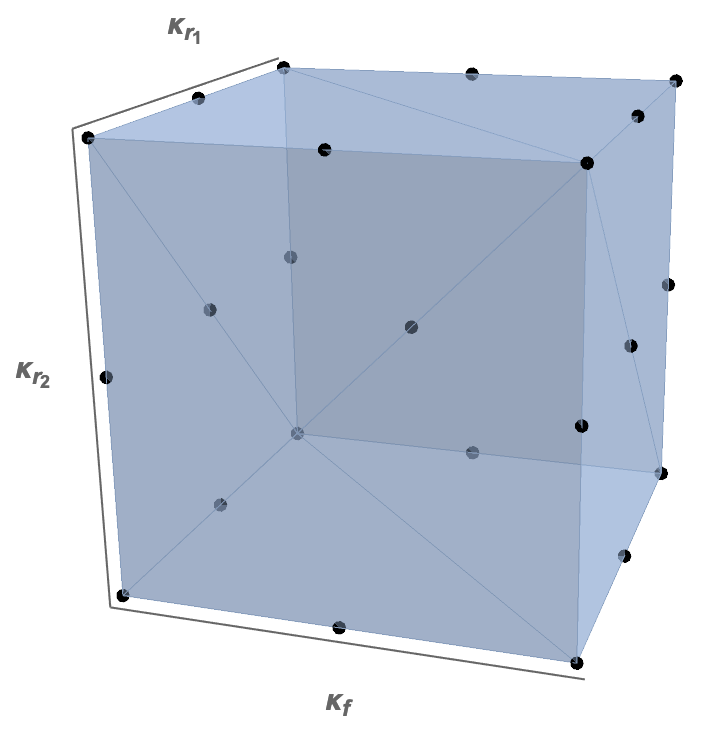
\includegraphics[scale=0.29]{9pt_3D.png}
    \begin{caption}{9-points prescription for a single process (left) and for two different processes $\pi_1$
        and $\pi_2$, indicating
        the sampled values for the factorization scale $\kappa_f$ and 
        renormalization scale $\kappa_r$.
    \label{fig:symmetricPrescriptions}
      }
    \end{caption}
    \end{figure}

    \section{Construction and validation of a theory covariance matrix}
    In this section we determine the theory covariance matrix at NLO using Eqs.~\ref{9S}, \ref{9M}
    and we validate it against the known NNLO results.
    As input datasets, we use the same NNPDF3.1 baseline given in Tab.~\ref{tab:experiments_chi2} with two minor differences:
    the value of the lower kinematic cut has been increased from $Q^2_{min} = 2.69 \,\,GeV^2$ to $13.96 \,\, GeV^2$
    in order to ensure the validity of the perturbative QCD expansion when scales are varied downwards, 
    and the HERA $F^b_2$ and fixed-target Drell-Yan cross-sections have been removed, 
    for technical reasons related to difficulties in implementing scale variation. 
    In total we then have $N_{dat} = 2819$ data points.
    As seen in the previous section, we assume that renormalization scale variation is fully correlated within 
    a given process, but uncorrelated between different processes.
    Having defined the input experimental data it is then necessary to define what we mean by "process" and
    divide the input dataset accordingly.
    Our categorization, summarized in Tab.~\ref{eq:expclassification}, involves five distinct processes:  charged-current (CC)
    and neutral-current (NC) deep-inelastic scattering (DIS),
    Drell–Yan (DY) production of gauge bosons (invariant mass,
    transverse momentum and rapidity distributions), single-jet
    inclusive and top pair production cross-sections.
    Note that such categorization requires and educated guess as to which theory computations share the same higher order
    corrections, and different choices might be done. 
    We consider the one presented here to be sufficient for a first study. 
    %
    In order to evaluate the theory covariance matrix $S_{ij}$, it is necessary
    to be able to evaluate both DIS structure functions and hadronic
    cross-sections for a range of values of the factorization
    and renormalization scales, i.e.for $k_f \neq  0$ and $k_r \neq 0$.
    %
    In this case, the entries of the NLO theory covariance matrix have been 
    constructed
    by means of the {\tt ReportEngine} software~\cite{zahari_kassabov_2019_2571601}
    taking the
    scale-varied NLO theory cross-sections $T_i(k_f,k_r)$  as input.
    %
    These are provided 
    by {\tt APFEL}~\cite{Bertone:2013vaa} for the DIS structure functions
    and by {\tt APFELgrid}~\cite{Bertone:2016lga} combined with
    {\tt APPLgrid}~\cite{Carli:2010rw} for the hadronic
    cross-sections.

    \begin{table}[t]
        \centering
        \renewcommand*{\arraystretch}{1.3}
        \begin{tabular}{|c|c|}
          \hline
          Process Type  & Datasets \\
          \hline
          DIS NC  &   NMC, SLAC, BCDMS, HERA NC \\
          DIS CC  &   NuTeV, CHORUS, HERA CC \\
          DY  & CDF, D0, ATLAS, CMS, LHCb ($y$, $p_T$, $M_{ll}$) \\
          JET  & ATLAS, CMS inclusive jets \\
          TOP  & ATLAS, CMS total+differential cross-sections \\
          \hline
        \end{tabular}
        \caption{\label{eq:expclassification}
         Classification of  datasets into  process types.
        }
    \end{table}
    %
    In order to get an idea of the structure of the theory-induced correlations,
    in Fig.~\ref{fig:covmats} we compare the experimental correlation matrix, given by
    \begin{align}
        \rho^{(C)}_{ij} = \frac{C_{ij}}{\sqrt{C_{ii}}\sqrt{C_{jj}}}\,,
    \end{align}
    with the corresponding combined experimental and theoretical correlation matrix
    \begin{align}
        \rho^{(C+S)}_{ij} = \frac{\left(C+S\right)_{ij}}{ \sqrt{\left(C+S\right)_{ii}} \sqrt{\left(C+S\right)_{jj}} }\,.
    \end{align}
    By inspection of Fig.~\ref{fig:covmats} large positive correlations within individual experiments along 
    the diagonal blocks are apparent, particularly evident for DIS NC and DY data.
    Within the same process there are large correlations between experiments for the DY, jets and top data points 
    and large anticorrelations for the DIS NC points, while correlations and anticorrelations between different processes,
    despite being present, are generally weaker.

    \begin{figure}[t!]
    \begin{center}
        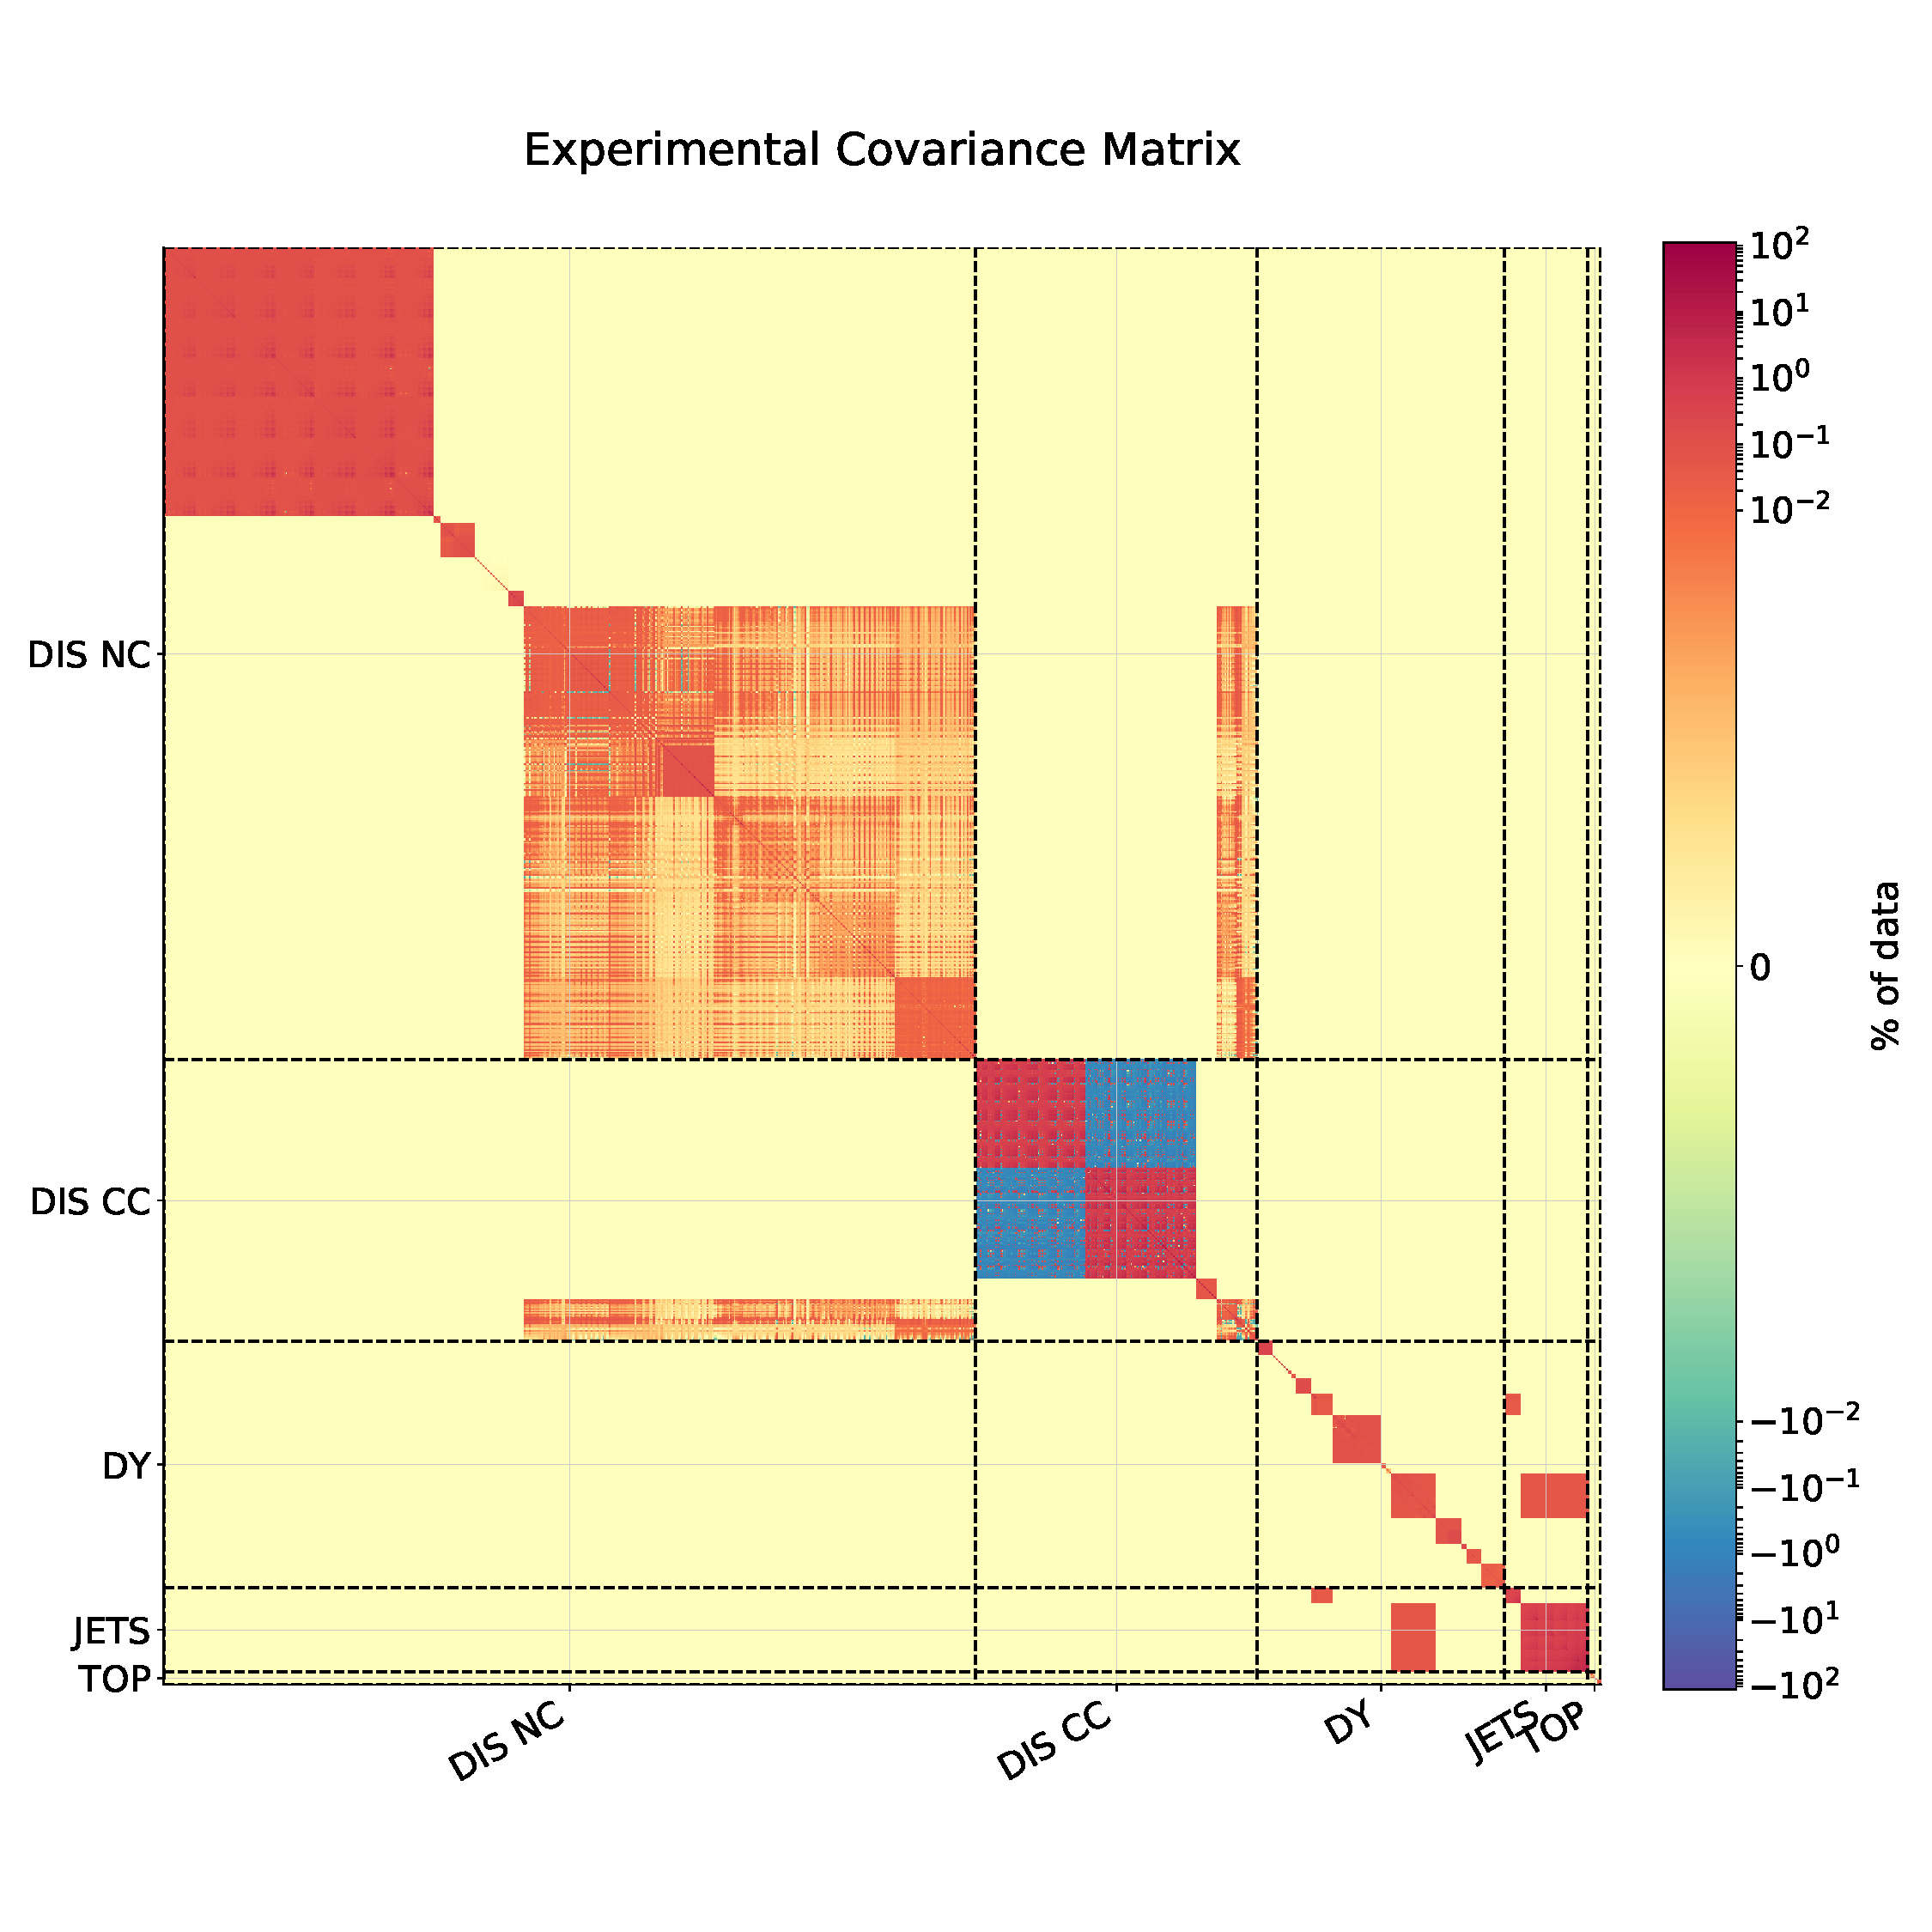
\includegraphics[width=0.49\linewidth]{exp_covmat.pdf}
        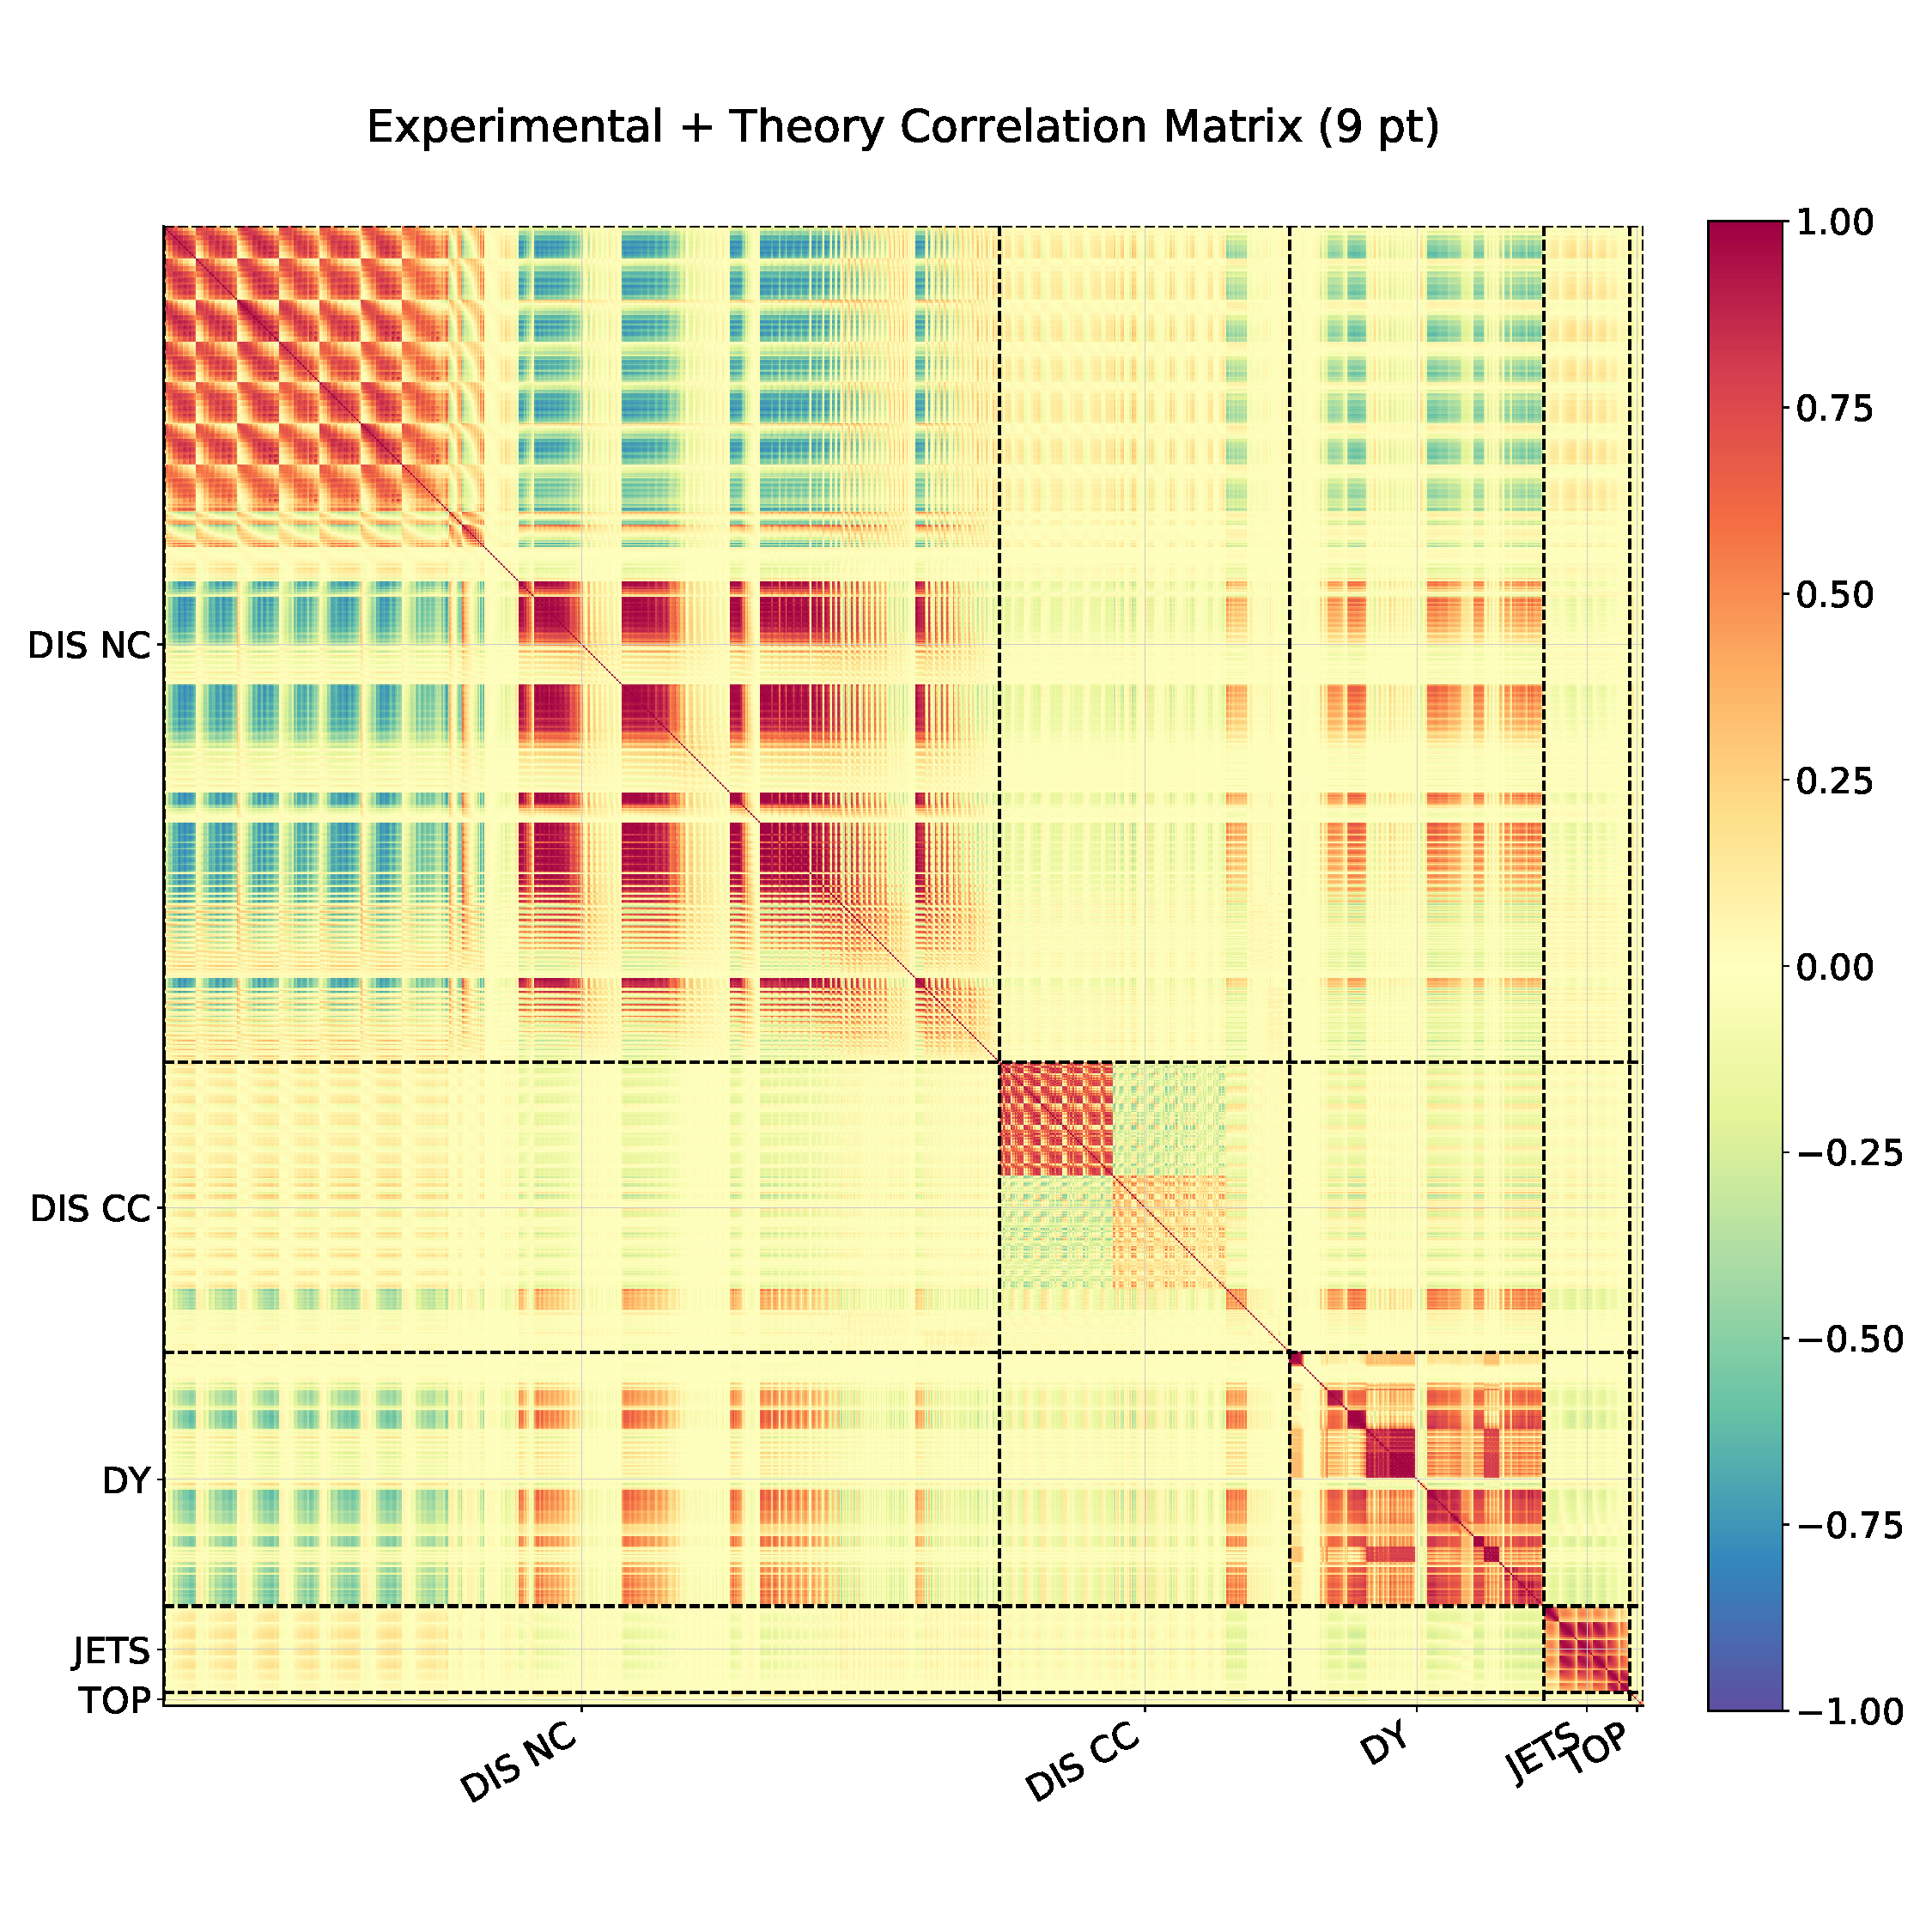
\includegraphics[width=0.49\linewidth]{expth_corrmat_9pt.pdf}
        \caption{\small Comparison of the  experimental $C_{ij}$ (left)
        and the and the the combined experimental and theoretical correlation matrices  $S_{ij}$, 
        the latter evaluated using the 9-point prescription.
        %
        All entries are normalized to the central  experimental value.
        %
        The data are grouped by process and, within a process, by experiment.} 
        \label{fig:covmats}     
    \end{center}
    \end{figure}

    
    %
    Next, we wish to construct a validation test for tye NLO theory covariance matrix, using the known shift between
    NNLO and NLO results.
    In order to do this, we view the set of experimental data as a vector $D_i$, where $i = 1, ..., N_{dat}$.
    Such vector lives in a $N_{dat}-$dimensional vector space $D$ and
    the theory covariance matrix $S_{ij}$ defines an ellipsoid $E$ belonging to a subspace $S$ of dimension
    $N_{sub}$ of the full space $D$. 
    %
    In the context of MHOUs we can take the NLO theory predictions evaluated at the central scales $T_i^{NLO}\left(0,0\right)$
    as our best NLO predictions with the ellipsoid $E$ estimating a $68\%$ confidence level for the MHO corrections. 
    We want to check how well $S_{ij}$ predicts both the size and the correlation pattern
    of the MHO terms. This can be done by testing the extend by which the known shift vector between NNLO and NLO theory predictions
    $T_i^{NNLO} - T_i^{NLO}$
    falls within the ellipsoid $E$.
    %
    More in detail, we first normalize the theory covariance matrix $S_{ij}$ to the NLO predictions, so that all its
    entry are dimensionless allowing for a meaningful comparison 
    \begin{align}
        \hat{S}_{ij} = S_{ij}/\left(T_i^{NLO}T_j^{NLO}\right)\,,
    \end{align}
    and likewise we define a normalized shift vector as
    \begin{align}
        \delta_i = \left(T_i^{NNLO}-T_i^{NLO}\right)/T_i^{NLO}\,.
    \end{align}
    The NNLO predictions used to define the shift are computed using the NNLO matrix elements and anomalous dimension
    but the same NLO PDF set used to compute the NLO theory predictions. In this way the shift $\delta_i$ 
    only accounts for the perturbative effects due to NNLO corrections, without including additional effects
    due to refitting.
    A first test to check whether the overall size of the scale variation is of the right order of magnitude
    consists into comparing the diagonal entries $\hat{S}_{ii} = \sigma_i^2$ to the normalized shift $\delta_i$.
    This check is performed in Fig.~\ref{fig:diag_shift_validation_symmetric}: in all cases 
    $\delta_i$ turns out to be smaller or comparable to $\sigma_i$, showing how how
    the overall size of the estimated uncertainties, obtained by varying the renormalization and factorization scales by
    a factor two in either directions, give a qualitative reliable (if somewhat conservative) estimate of the true MHOU. 
    \begin{figure}[t!]
        \begin{center}
          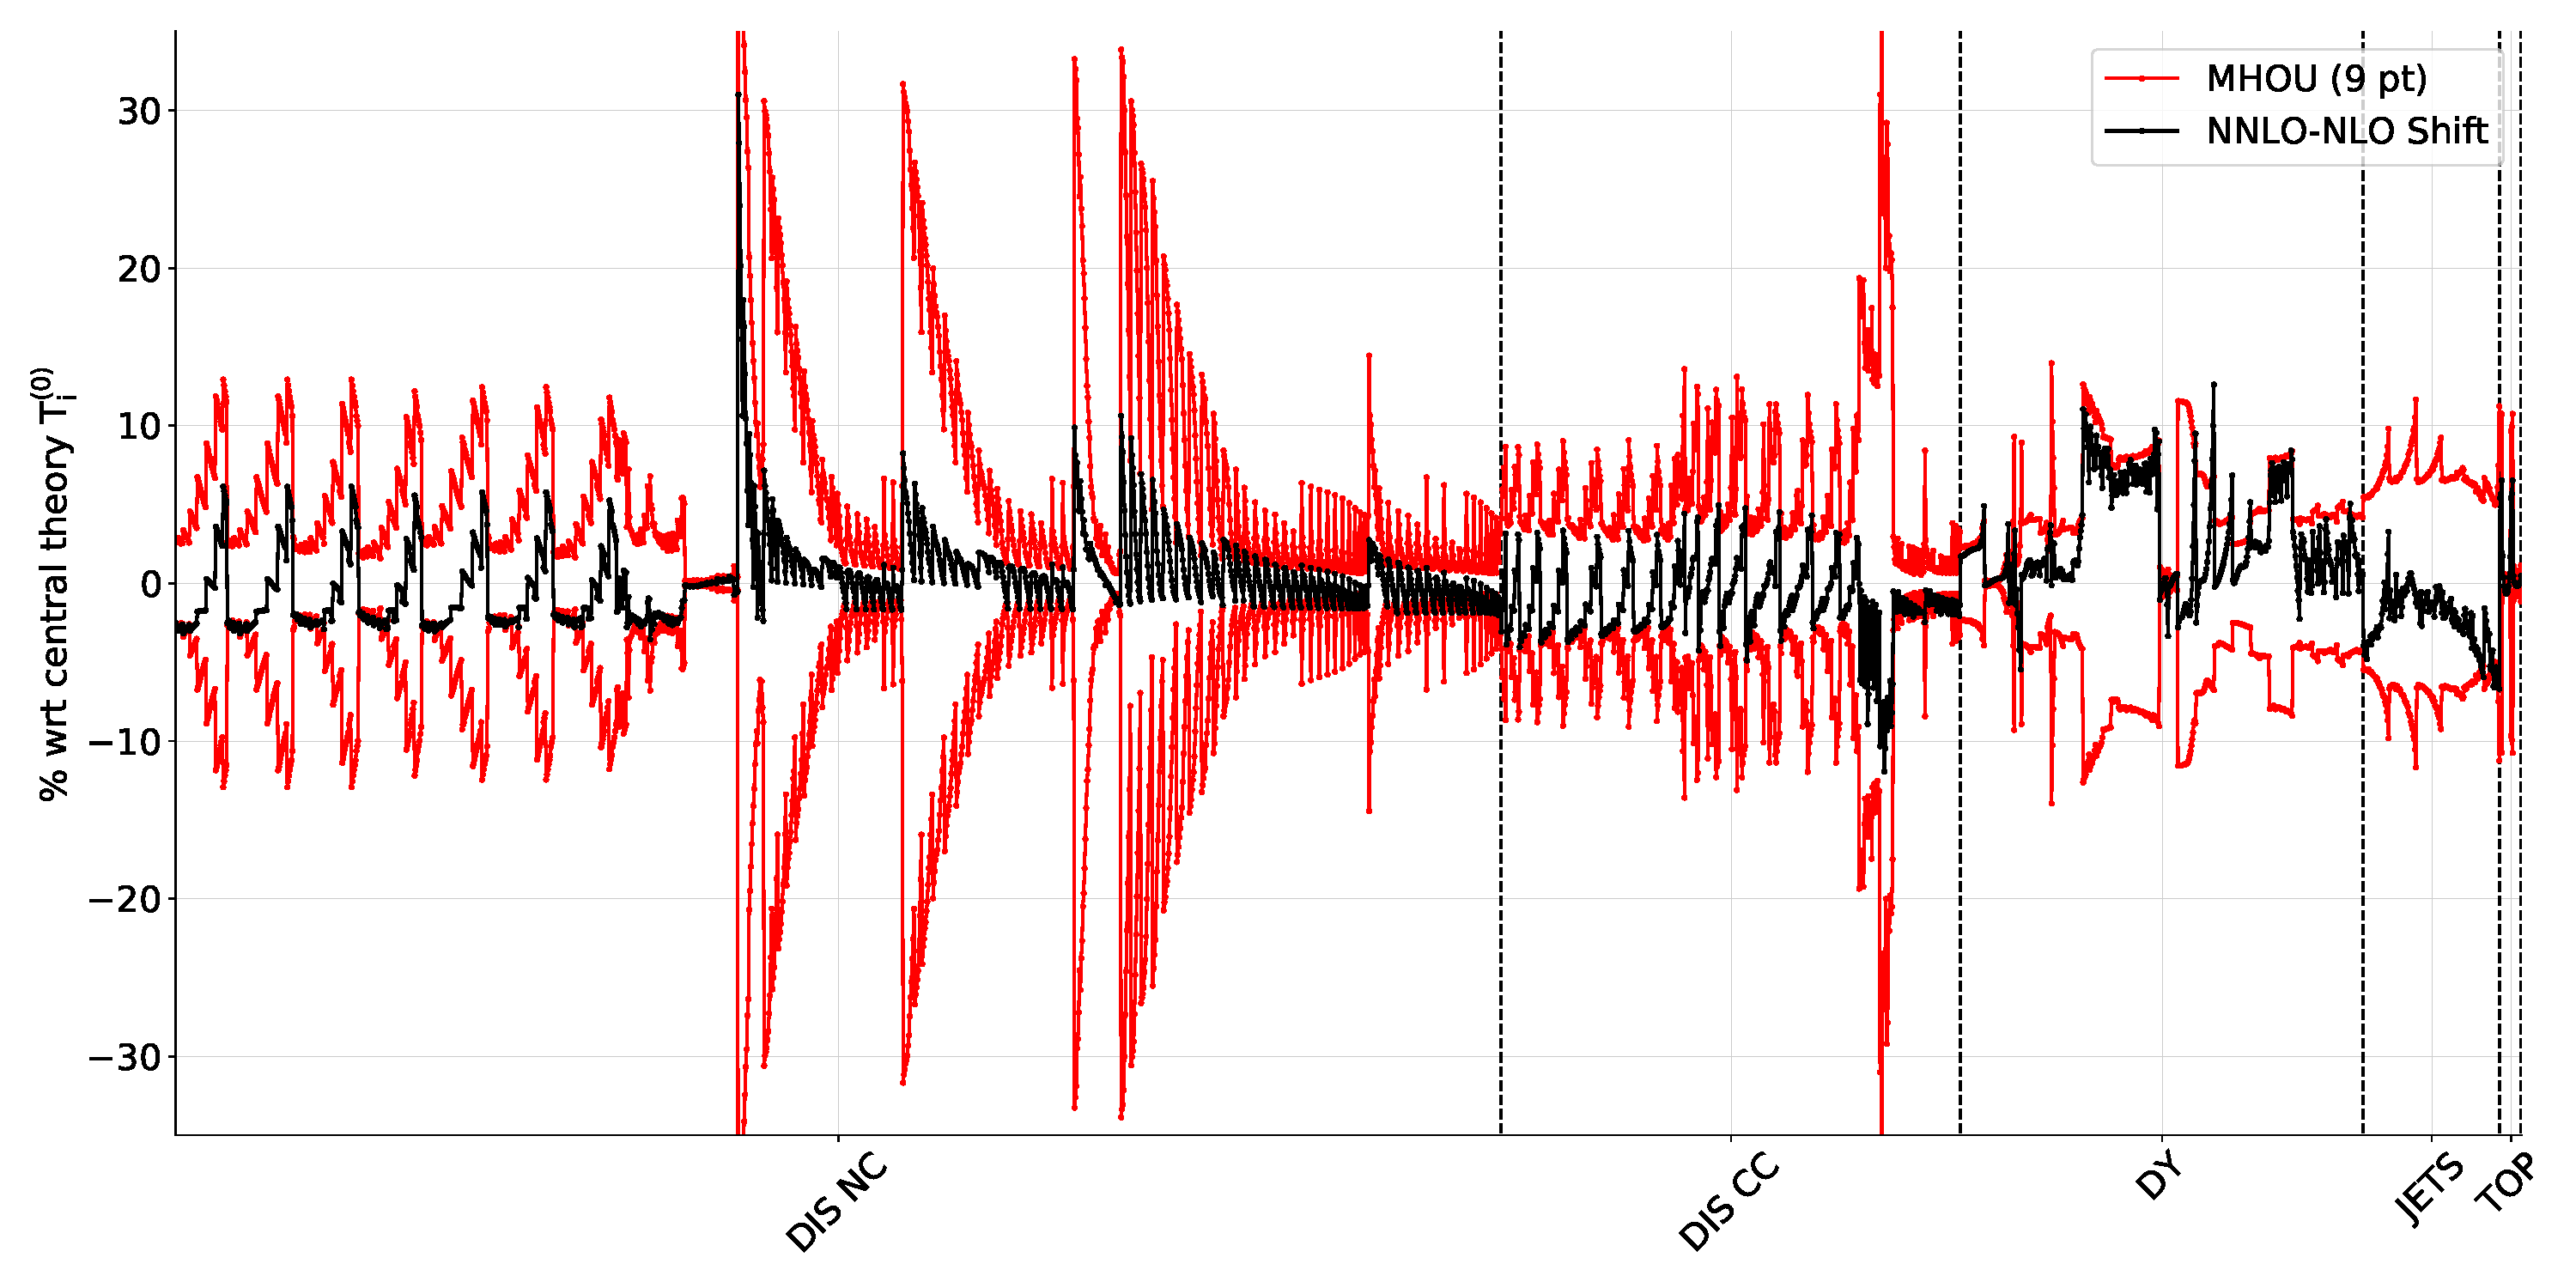
\includegraphics[width=14cm, height=4.4cm]{shift_diag_cov_comparison_9pt_global.pdf}
          \caption{\small The diagonal uncertainties  $\sigma_i$ (red)
            symmetrized about zero,
            compared to the shift $\delta_i$ (black) for each
            datapoint.}
          \label{fig:diag_shift_validation_symmetric}
        \end{center}
    \end{figure}

    The validation of the full covariance matrix $\hat{S}_{ij}$ requires some more work.
    In order to identify the subspace $S$ we diagonalize the matrix $\hat{S}_{ij}$, getting a set
    of orthonormal eigenvectors $e_i^{\alpha}$ and the corresponding non-zero eigenvalues 
    $\lambda_{\alpha}$ with $\alpha = 1, ..., N_{sub}$.
    There is also a set of $N_{dat}-N_{sub}$ zero eigenvalues, corresponding to eigenvectors spanning
    the space $D/S$.
    In general the shift vector $\delta$ will live in the space $D$. 
    For a successful test we expect most of $\delta$ to lie within $S$.
    In other words, denoting as $\delta^s$ the projection of the shift over the subspace $S$
    \begin{align}
        \delta_i^s = \sum_{\alpha=1,...,N_{sub}} \delta^{\alpha}e^{\alpha}_i\,,
    \end{align} 
    we expect the angle $\theta$ between $\delta$ and $\delta^s$
    \begin{align}
        \theta = \arccos\left(\frac{|\delta_i^s|}{|\delta_i|}\right)
    \end{align}
    to be reasonably small. This geometric relation is represented graphically in Fig.~\ref{fig:subspace_diagram},
    where the space $D$ is drawn as a three dimensional space and the subspace $S$ as a two dimensional space.
    For individual processes we find $\theta = 3^{\rm o}, 14^{\rm o}, 22^{\rm o}, 32^{\rm o}, 16^{\rm o}$ for top, jets, DY, NC and CC DIS respectively, 
    while the complete dataset we find $\theta = 26^{\rm o}$.
    %
    \begin{figure}[t]
        \begin{center}
          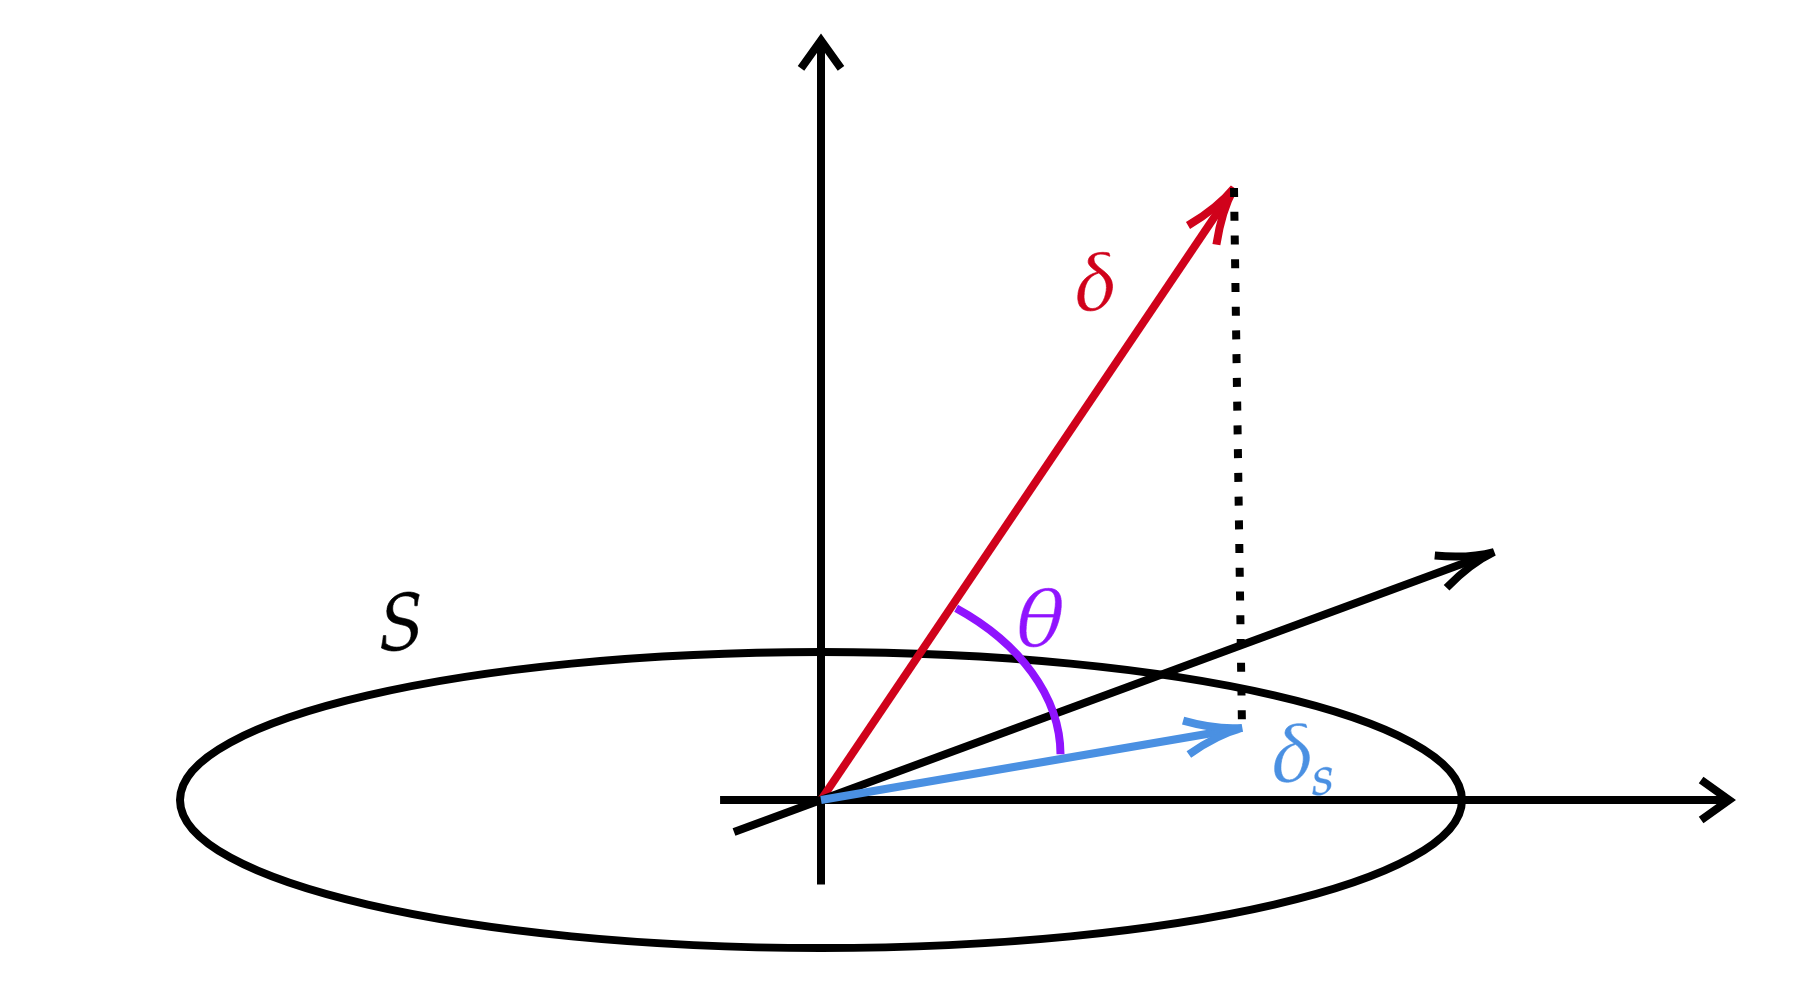
\includegraphics[scale=0.12]{subspace_diag.png}
          \caption{\small Schematic representation of the geometric relation
            between the shift vector $\delta\in D$ (here drawn as a three dimensional space), and
            the component $\delta^S$ of the shift vector which lies in the 
      subspace $S$ (here drawn as a two dimensional space, containing the ellipse E defined by the theory covariance matrix). 
      The angle $\theta$ between $\delta$ and $\delta^S$ is also shown.
          \label{fig:subspace_diagram} }
        \end{center}
      \end{figure}
    %
    It is clear from these numbers how processes with larger numbers of data points, having 
    a wider kinematic range and thus more structure to predict, are much harder to describe than those 
    with only few data, which translates into bigger values of $\theta$ for bigger datasets. However in general the
    $\theta$ values we get for each specific process and for the global dataset result reasonably small, validating our definition
    and construction of a NLO theory covarinace matrix.

    \section{NLO PDFs with missing higher order uncertainties}

    